\documentclass[a4paper,12pt,final]{report}
\usepackage[margin=0.8in]{geometry}
% Pour une impression recto verso :
%\documentclass[a4paper,11pt,twoside,final]{article}
%%%%% Packages %%%%%
\usepackage[french]{babel}  % Rapport en français
\usepackage[utf8]{inputenc}   % UTF-8 forever <3
\usepackage[T1]{fontenc}      % font encoding (allows accents)
\usepackage[pdftex]{graphicx} % gestion des images
\usepackage{setspace}         % gestion des interlignes
\usepackage{csquotes}         % For quotes
\usepackage[hidelinks]{hyperref}         % gestion des url
\usepackage{titlesec}         % override chapter title
\usepackage{geometry}         % gestion des marges
\usepackage{float}            % Gestion des positionnement d'image
\usepackage[final]{pdfpages}  % Inclusion de fichier pdf
\usepackage{framed}
\usepackage{geometry}
%\usepackage{apacite}

%%% Affichage de code
\usepackage{listings}
\usepackage{xcolor}
\usepackage{textcomp}
% 添加首行缩进,两个字符
\usepackage{indentfirst}
\usepackage[bottom]{footmisc}

\setlength{\parindent}{2em}

\definecolor{comment}{rgb}{0.12, 0.38, 0.18 } % adjusted, in Eclipse: {0.25, 0.42, 0.30 } = #3F6A4D
\definecolor{keyword}{rgb}{0.37, 0.08, 0.25}  % #5F1441
\definecolor{string}{rgb}{0.06, 0.10, 0.98} % #101AF9
\lstset{
  columns=flexible, %prevent extra spaces
  rulecolor=\color{black!50},
  backgroundcolor = \color{blue!10},
  numbers=none, % line numbering
  showspaces=false,
  showtabs=false,
  tabsize=2,
  breaklines=true,
  showstringspaces=false,
  breakatwhitespace=false,
  commentstyle=\color{comment},
  keywordstyle=\color{keyword},
  stringstyle=\color{string},
  basicstyle=\ttfamily,
  extendedchars=true,
  emph=[2]{In},
  emphstyle=[2]\color{black!70},
  morecomment=[l][\color{blue}]{Out},
  frame=single,
  frameround=tttt,
  framerule=0.3pt,
  framesep=4pt,
  belowcaptionskip=2.1pt,
  literate={à}{{\`a}}1 {à }{{\`a} }1 {â}{{\^a}}1 %           letter a
           {À}{{\`A}}1 {Â}{{\^A}}1 %                         letter A
           {ç}{{\c{c}}}1 %                                   letter c
           {Ç}{{\c{C}}}1 %                                   letter C
           {é}{{\'e}}1 {è}{{\`e}}1 {ê}{{\^e}}1 {ë}{{\"e}}1 % letter e
           {É}{{\'E}}1 {È}{{\`E}}1 {Ê}{{\^E}}1 {Ë}{{\"E}}1 % letter E
           {î}{{\^i}}1 {ï}{{\"i}}1 %                         letter i
           {Î}{{\^I}}1 {Ï}{{\"I}}1 %                         letter I
           {ô}{{\^o}}1 %                                     letter o
           {Ô}{{\^O}}1 %                                     letter O
           {œ}{{\oe}}1 %                                     letter oe
           {Œ}{{\OE}}1 %                                     letter OE
           {ù}{{\`u}}1 {û}{{\^u}}1 {ü}{{\"u}}1 %             letter u
           {Ù}{{\`U}}1 {Û}{{\^U}}1 {Ü}{{\"U}}1 %             letter U
  % above is a hack to force UTF8 compatibility (only for french)
}
%%% Bibliographie
\usepackage[backend=biber,style=numeric-comp]{biblatex}
\addbibresource{bibliographie.bib}
%\bibliographystyle{plain}
%\bibliography{bibliographie}
%%%%% Configuration %%%%%
\definecolor{shadecolor}{gray}{0.9}

%\pagenumbering{arabic}
% Numérotation des figures sans la référence à la partie
\renewcommand{\thefigure}{\arabic{figure}}
\counterwithout{figure}{chapter}
% A TESTER
\counterwithout{table}{chapter}
\counterwithout{footnote}{chapter}
%%% Quelques champs
\newcommand{\reportsubject}{Développement de l'interface homme-machine pour l'inspection automatisée}  % Internship purpose
\newcommand{\reportauthor}{Zhentao \textsc{XU}} % Author
\newcommand{\reportdates}{13 février 2023 - 28 juillet 2023} %Internship dates
\newcommand{\reporttitle}{Rapport de stage - TN09 - GI} % Title
\renewcommand\labelitemi{---} %list items hyphens rather than nodes
\renewcommand{\contentsname}{Sommaire} % Nom table des matières
%%% Inline comment
\newcommand{\ignore}[1]{}

%%% Modification de style pour \chapter
\titleformat{\chapter}{\normalfont\huge}{\textbf{\thechapter.}}{20pt}{\huge\bf}

%%% Marges
\geometry{hmargin=2.45cm}

% Set line width
\newcommand{\HRule}{\rule{\linewidth}{0.5mm}}
% Espace entre les paragraphes
\setlength{\parskip}{1ex}

%% ToC Name :

\addto\captionsenglish{
  \renewcommand{\contentsname}
    {Sommaire} 
    \renewcommand{\listfigurename}{Table des figures}
}

%%% Meta-données
\hypersetup{
    pdftitle={\reporttitle},%
    pdfauthor={\reportauthor},%
    pdfsubject={\reportsubject},%
    colorlinks=false,% hyperlinks will be black
    linkbordercolor=black,% hyperlink borders will be black
    pdfborderstyle={/S/U/W 1}% border style will be underline of width 1pt
}

%% Table of content configuration
\setcounter{tocdepth}{1}


\usepackage[toc,section=chapter]{glossaries}    % Glossaire

\makeglossaries


\newglossaryentry{IDE}
{
	name=\underline{IDE},
	description={\textit{Integrated Development Environment} en français :  Environnement de Développement Intégré (EDI) }
}

\newglossaryentry{LaTeX}
{
	name=\underline{LaTeX},
	description={LaTeX est un langage de description donnant à l'auteur les moyens d'obtenir des documents mis en page de façon professionnelle sans avoir à se soucier de leur forme. La priorité est donnée à l'essentiel : le contenu (c.f \underline{\href{https://openclassrooms.com/fr/courses/1617396-redigez-des-documents-de-qualite-avec-latex/1617565-quest-ce-que-latex}{OpenClassrooms}})}
}

\newglossaryentry{SmartSVN}
{
	name=\underline{SmartSVN},
	description={logiciel de gestion de versions décentralisé. C'est un logiciel libre créé par Linus Torvalds, auteur du noyau Linux, et distribué selon les termes de la licence publique générale GNU version 2.  (c.f \underline{\href{https://fr.wikipedia.org/wiki/Git}{Wikipédia}})}
}


\newglossaryentry{API}
{
	name=\underline{API},
	description={\textit{Application Programming Interface }, Interface de Programmation Applicative, permettant à un logiciel d'offrir un accès facilité à certaines de ses fonctions, méthodes et classes}
}



\glsaddall
\renewcommand*{\glstextformat}[1]{\textbf{#1}}
\makeglossaries
\pagenumbering{gobble}
%%%%% Début du document %%%%%
\begin{document}
\nocite{*}

\makeatletter
  \begin{titlepage}
    \centering
    \noindent
\includegraphics[height=0.8cm]{ressources/images/deltacad_logo.png}\hfill
\includegraphics[height=1cm]{ressources/images/utc_logo.png}\\
    \vfill

    \textsc{\Large \reporttitle}\\[0.5cm]
    \HRule \\[0.4cm]
    {\huge \bfseries \reportsubject}\\[0.5cm]
    \HRule \\[1.5cm]
    \textsc{\large \reportdates}\\[0.5cm]

    \vfill

    \begin{minipage}[t]{0.3\textwidth}
      \begin{flushleft} \large
        \emph{Auteur :}\\
        \reportauthor
      \end{flushleft}
    \end{minipage}
    \begin{minipage}[t]{0.6\textwidth}
      \begin{flushright} \large
        \emph{Encadrant UTC :} \\
		Véronique \textsc{CHERFAOUI} \\
        ~\\
		\emph{Encadrant entreprise :} \\
		Julien \textsc{MONVILLE} \\
        ~\\
        \emph{Entreprise :} \\
		Deltacad\\
        795 rue de Longues Rayes\\
        60610, Lacroix Saint-Ouen\\
      \end{flushright}
    \end{minipage}
  \end{titlepage}

\makeatother
\setstretch{1,3}
\pagenumbering{arabic}
\chapter*{Remerciements} %the * make the chapter invisible in the table of content

Je tiens à remercier toutes les personnes qui ont contribué au succès de mon stage et qui m'ont aidé lors de la rédaction de ce rapport.  \\

Tout d'abord, je tiens à remercier vivement Vincent ARGENTON, mon maitre de stage, pour le temps qu'ils m'a toujours accordé sans hésitation, ainsi que pour les opportunités et responsabilités qu'il m'a offertes. \\

Ensuite, je voudrais remercier le manager de l'équipe, Stéphane GLOAGUEN, pour la reconnaissance, le temps et les conseils qu'il m'a accordé. \\
	
De plus, je souhaite aussi remercier Kevin HELOUART, qui, avec Vincent, a su m'intégrer à l'équipe très rapidement.  \\

Enfin, je remercie Michelangelo NERI et Milan RADOVIC d'avoir accepté ma candidature.\\

Je souhaite aussi remercier tout mes collègues pour le temps passé à leurs côtés, ainsi que pour leurs précieux conseils, et plus spécialement Thibault, Bastien et Dominique.
\setstretch{1,15}
\tableofcontents
\chapter*{Table des figures} %the * make the chapter invisible in the table of content
\addcontentsline{toc}{chapter}{Table des figures}

\begin{itemize}
\item \textbf{Figure 1 :} Prototype d’interface PowerEye - page 9
\item \textbf{Figure 2 :} Interface PowerEye redessinée - page 9
\item \textbf{Figure 3 :}  La liaison de données - source : https://learn.microsoft.com/en-us/dotnet/desktop/wpf/data/?view=netdesktop-7.0 - page 14
\item \textbf{Figure 4 :} La structure globale du PowerEye - page 14
\item \textbf{Figure 5 :} La structure des données du PowerEye - pages 15
\item \textbf{Figure 6 :} La Conception initiale de l’interface - page 16
\item \textbf{Figure 7 :} La disposition finale de l’interface - page 17
\item \textbf{Figure 8 :} la fenêtre principale - page 17
\item \textbf{Figure 9 :} l’interface graphique d’extraction d’images - page 18
\item \textbf{Figure 10 :} l’interface graphique d’ajout du bruit- page 19
\item \textbf{Figure 11 :} deux paramètres d’entrée- page 20
\item \textbf{Figure 12 :} Interface graphique d’apprentissage automatique - page 21
\item \textbf{Figure 13 :} Interface graphique de la surveillance de la ligne d’assemblage - page 22
\item \textbf{Figure 14 :}  Interface graphique pour le stockage des données relatives aux pièces - page 23
\item \textbf{Figure 15 :} Interface graphique pour la vérification manuelles - page 23
\item \textbf{Figure 16 :} Interface graphique pour l’interrogation de l’historique - page 24
\item \textbf{Figure 17 :} Interface graphique montrant la configuration globale - page 25
\item \textbf{Figure 18 :} Interface graphique pour appliquer la configuration - page 26
\item \textbf{Figure 19 :} Fonctionnalité de configuration appliquée à des interfaces individuelles - page 26
\item \textbf{Figure 20 :} Interface graphique pour des flux de travail personnalisés - page 27
\item \textbf{Figure 21 :}  Affichage de l’appel de fonction - page 28
\end{itemize}
\setstretch{1,3}
\chapter*{Résumé technique}
\addcontentsline{toc}{chapter}{Résumé technique}

Mon stage se déroule à Deltacad, une société d’ingénierie spécialisée en informatique scientifique. En collaboration avec une entreprise AML System et deux instituts de recherche, les laboratoires Roberval et Heudiasyc de l’UTC, nous développons un logiciel pour des scénarios industriels, qui entraîne des modèles d’apprentissage automatique à partir d’images de pièces sur la chaîne de production et les applique pour déterminer la qualité des pièces et détecter les défauts.\\

Dans ce cadre, ma tâche consistait à concevoir et à développer l'interface homme-machine et à améliorer progressivement sa fonctionnalité en fonction des besoins.
Durant mon stage, J'ai réalisé une interface du logiciel extensible en utilisant WPF et j'ai conçu l'architecture globale du logiciel, en intégrant des modules fonctionnels déjà conçus ainsi que certains de mes propres modules fonctionnels. Par ailleurs, j'ai également utilisé certaines extensions externes, telles que l'affichage des journaux d'opérations via le cadre POA (programmation orientée aspect), et l'enregistrement et l'importation des informations de configuration via la sérialisation xml.\\

\vspace{1\baselineskip}

\noindent Mots-clés : .Net WPF, MVVM(Model-View-ViewModel), C\#, POA, python, C++
\chapter*{Introduction}
\addcontentsline{toc}{chapter}{Introduction}

Dans le cadre de ma formation d’ingénieur à l’Université de Technologie de Compiègne, le troisième semestre est consacré à un stage de 24 semaines d’assistant ingénieur. Cette expérience comme une longue période de travail professionnel, nous permet d’avoir un aperçu du fonctionnement de l’entreprise et du monde professionnel, d’appliquer les connaissances acquises lors de sa formation, d’exprimer notre créativité et nos idées jeunes et énergiques. Et dans ce rapport de stage, je résume le travail que j'ai effectué à Deltacad au cours des six mois allant de février 2023 à juillet 2023 et je le présente plus en détail en trois partis principaux.\\

Dans la première partie, je vous donnerai une vue d'ensemble de mon entreprise et mon point de vue sur mon équipe. Cela vous donnera un premier aperçu de l'environnement de mon stage.\\

Dans la deuxième partie, je vous présenterai quelques détails sur l'ensemble de mon stage, y compris le sujet du stage, l'organisation des tâches, ma contribution et les aspects techniques du projet. En résumé, cette section est plus orientée vers une vision globale et n'est pas divisée en modules individuels.\\

Dans la troisième section, je décomposerai mes réalisations au cours de mon stage en un certain nombre de points afin de les expliquer plus en détail. Je également expliquerai les raisons pour lesquelles j'ai choisi certaines options, ainsi que les difficultés et solutions techniques rencontrées à ce moment-là. Dans cette partie, je me concentrerai sur les aspects techniques et, en raison de la spécificité du projet, je parlerai des différents modules du projet pour vous donner une compréhension plus claire.\\

Enfin, je résumerai les améliorations que j'ai apportées pendant mon stage et je donnerai quelques indications sur le développement futur du projet. 

\chapter{Présentation de Deltacad}
\section{Présentation génerale}
La société Deltacad, basée à Compiègne, est spécialisée, depuis plus de 20 ans, dans la conception, la réalisation, la maintenance et la diffusion d'applications scientifiques et techniques, ainsi que la réalisation d'études avancées s'appuyant sur l'utilisation des logiciels développés.
Les clients de Deltacad sont majoritairement des grands groupes industriels ou des collectivités/institutionnels répartis dans 4 grands secteurs équilibrés :
\begin{itemize}
\item Environnement: CEREMA, DREAL, EPLoire, EPAMA, BRGM, Vendée-Eau, 
Oise-Aisne.
\item Energie et génie civil: AREVA, CEA, CERN, EDF, ENGIE, GRTGaz, EGIS,
Vallourec, Fondation Louis Vuitton, Setra, Vinci, TRACTEBEL, ...
\item Aéronautique, ferroviaire et naval: AIRBUS,
COMAC, DAPA, Dassault Aviation, MBDA, SAFRAN, STELIA, ...; ALSTOM,
SNCF ; AGCO (Challenger, Fendt, ...) ; Caterpillar, Volvo, ...
\item Automobile: Constructeurs automobile (PSA, BMW, ...) ; équipementiers 
(SOGEFI, Saint Gobain, Valéo, Delphi, ...) ; Sidérurgie (ArcelorMittal, Corus, Nippon Steel, ...) 
\end{itemize}
Deltacad noue également de forts partenariats avec des équipes universitaires : UTC dans le cadre du laboratoire commun DIMEXP, UTBM, UTT, ECN, ENSAM, INSA, dans le cadre de projets R\&D. 
Les équipes de Deltacad sont ainsi régulièrement enrichies des compétences de stagiaires et d'alternants des différentes universités partenaires, pour mener à bien des projets à fort potentiel d'innovation.

\newpage
\section{Les produits}
Deltacad assure le développement et le support de différents logiciels :
\begin{itemize}
\item \textbf{Gamme DeltaMESH} : DeltaMESH est dédiée à la modélisation géométrique et au maillage de modèles surfaciques issus des logiciels de CAO. (“Nos produits – Deltacad.fr”) Le maillage consiste à transformer un modèle CAO en un objet tridimensionnel composé de polygones exploitable pour des applications de visualisation et/ou de simulation. Le logiciel autorise des maillages automatiques directement sur des modèles CAO en supprimant l’étape 
fastidieuse de nettoyage de ces modèles. DeltaMESH se décline en plusieurs 
produits, chacun répondant à un besoin particulier : DeltaMESH Stamping dédié 
à la simulation des process de fabrication (emboutissage, fonderie ...), 
DeltaMESH Fillet, outil de rayonnage automatique de maillages possédant des 
arêtes vives, DeltaMESH FEM, un mailleur permettant de générer des maillages 
de qualité "éléments finis" destinés à différents types de calculs (mécanique, thermique...).
\item \textbf{Osiris-inondations et Osiris-Multirisques} : Osiris-inondations est un outil d'aide à la réalisation de Plans Communaux de Sauvegarde (PCS) destinés aux élus locaux. Ses fonctionnalités vont de la simulation de la montée des eaux, à la gestion d'une situation de crise en cas d'inondation et jusqu'à la réalisation de plans d'interventions pour les communes touchées. Osiris-Multirisques étend ces possibilités aux risques naturels et technologiques.
\item \textbf{Code\_Aster} : Code\_Aster est un logiciel de simulation par éléments finis développé et utilisé par EDF pour ses études en mécanique des structures. Deltacad assure son développement et le support pour les utilisateurs de EDF.
\end{itemize}

\chapter{Mission}
\section{Sujet de stage}
Le sujet de mon stage était initialement \texttt{Développement/Intégration de fonctions de Vision par ordinateur pour l’inspection automatisée}. Durant toute la période de mon stage, mon travail s'est axé autour d'un logiciel appelé \texttt{PowerEye}. \texttt{PowerEye} est un logiciel développé pour des scénarios industriels qui utilise la vision par ordinateur pour détecter les défauts des pièces sur la chaîne de production. Les laboratoires de l’UTC faisant partie de ce projet, ils assurent le développement des machines apprenantes. Deltacad est responsable de la conception de l'interface de l'ensemble du projet et de l'intégration des autres fonctions. \\

Avant que je ne commence mon stage, \texttt{PowerEye} avait déjà été conçu avec certaines fonctionnalités ainsi qu'un prototype d'interface. Cependant, il était clair que le système n'était pas encore adapté à une application formelle au sein de l'entreprise. Par conséquent, la tâche principale de mon stage consistait à concevoir et améliorer une interface homme-machine plus pratique basée sur le prototype de l'interface et essayer de tester les pièces d'AML Systems\footnote{un société du segment éclairage du groupe Johnson Electric, conçoit, produit et commercialise, des solutions pour améliorer la visibilité, la sécurité, et le confort du conducteur} à l'aide de cette interface après intégration de la fonction.\\

En ce qui concerne les lignes directrices spécifiques pour la conception de l'interface, le chef de projet et le suiveur m'ont fourni un aperçu général des différents modules qu'elle contiendrait et des fonctionnalités qu'elle pourrait inclure. Après avoir confirmé le thème et le programme de travail, mon stage a officiellement commencé.\\

\newpage
\section{Planning de stage}
Au début de mon stage, mes tâches étaient planifiées en trois phases : 
\begin{itemize}
    \item \textbf{1. }Développement de l'interface homme-machine de PowerEye 
    \item \textbf{2. }Test sur les données de l'entreprise partenaire AML système
    \item \textbf{3. }Déploiement d'applications dans le système AML
\end{itemize}

Dans le cadre du travail réel, pour chaque phase de la tâche, je l'ai décomposée en différentes étapes. La première phase peut en fait être divisée en plusieurs parties : la conception de l'interface, la réalisation de l'apparence de l'interface, la réalisation de la structure des données de l'interface et la réalisation des fonctions de la couche d'application de l'interface. La deuxième phase comprend également l'intégration de la fonctionnalité conçue, le test des données et l'amélioration de la fonctionnalité. Il est très regrettable qu'en raison de contraintes de temps, mon stage se soit terminé à la deuxième phrase. Mais en fait, en plus des tâches incluses dans le plan, j'ai également complété un certain nombre d'autres fonctionnalités, y compris enregistrement des appels de fonction et exécution de programmes de script c\# via des chaînes de caractères\\

À mon avis, la partie la plus importante du processus de stage est la structure globale du projet, car elle influe grandement sur le développement des idées et l'évolutivité du projet. À cette fin, j'ai amélioré l'architecture globale à plusieurs reprises au cours du processus de développement, en utilisant des \texttt{prism} au début de projet individuel, en divisant l'interface en couches d'affichage et d'application, et en développant avec le cadre mvvm.



\newpage
\section{Contributions}
Comme mentionné dans la section précédente, lorsque j'ai commencé à travailler sur le projet, il existait déjà un prototype d'interface ainsi que certains modules fonctionnels.
\begin{figure}[H]
    \centering
    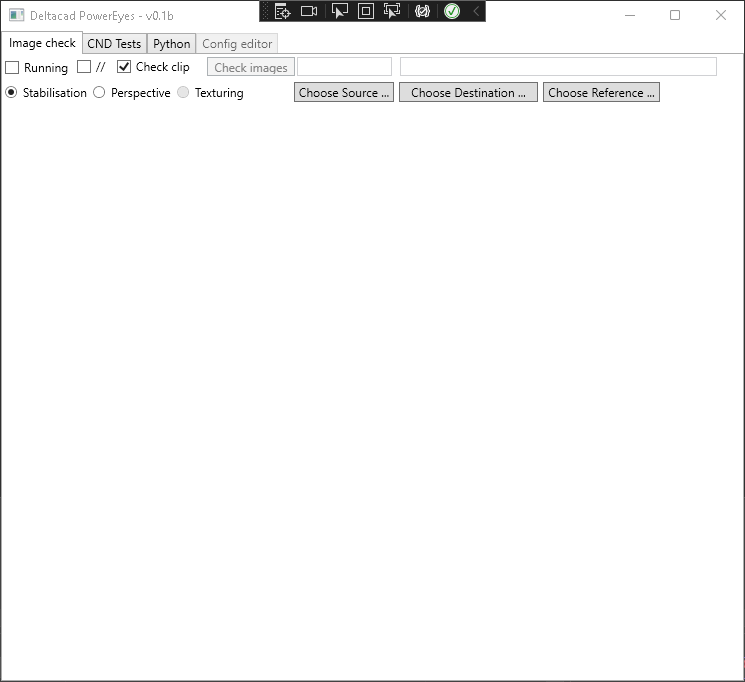
\includegraphics[height=5cm]{ressources/images/prototype.png}
    \caption{Prototype d'interface PowerEye}
\end{figure}
L'interface se compose de quatre modules: Image check, CND Tests, python et config editor. Il contient des méthodes d'application de de Template Matching pour la détection des pièces et des modèles d'entraînement pour les tests avec des ensembles de données.\\
Mais le fait est que l'interface prototype n'est pas suffisante pour inclure toutes les fonctionnalités envisagées par PowerEye. Par conséquent, ma principale contribution tout au long du stage a été la conception et le développement d'une nouvelle version de l'interface \texttt{PowerEye}. À la fin du stage, la nouvelle version de l'interface de powereye ressemblait à ceci. \\
\begin{figure}[h]
    \centering
    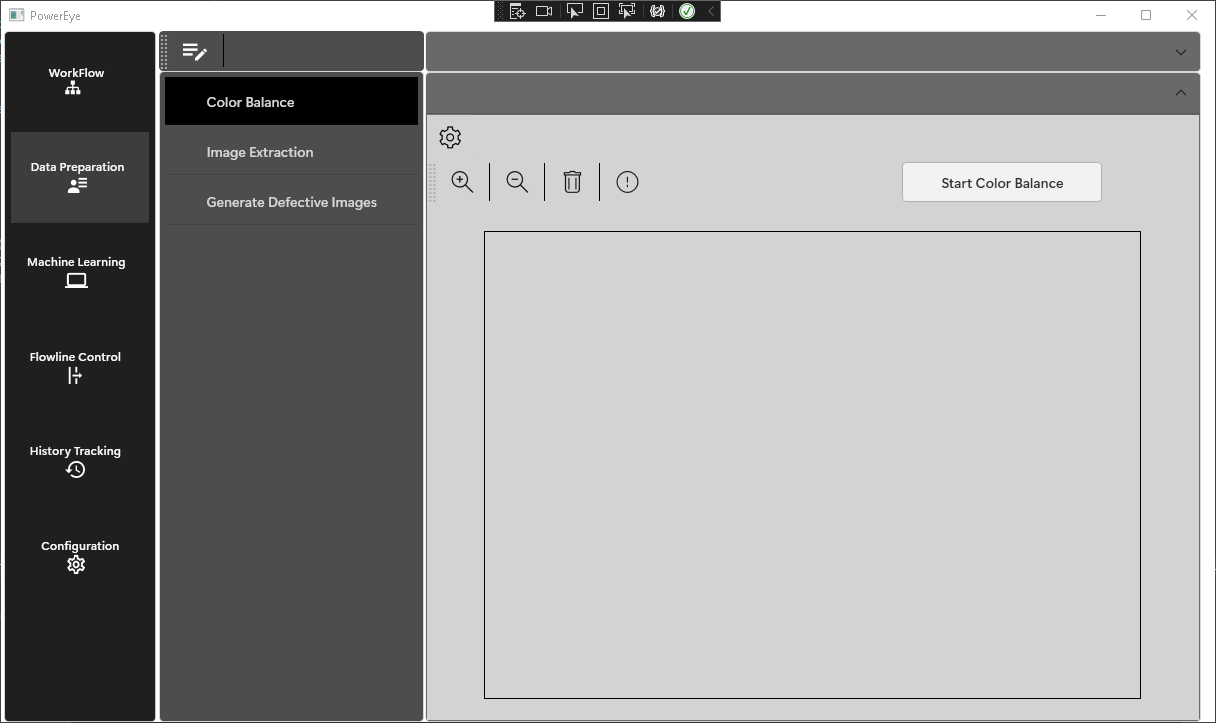
\includegraphics[height=6cm]{ressources/images/color_balance.png}
    \caption{Interface PowerEye redessinée}
\end{figure}
Il contient cinq modules : 
\begin{itemize}
    \item \textbf{Préparation des données (Data preparation): }Ce module permet d'extraire les contours des pièces de l'image et d'ajouter du bruit de perlin à l'image. 
    \item \textbf{Apprentissage automatique (machine learning): }Ce module est utilisé pour entraîner le modèle ckpt à partir de l'ensemble de données.
    \item \textbf{Contrôle de la chaîne d'assemblage (flowline control): } Ce module détecte si une pièce est qualifiée par Template Matching, et enregistre les données du résultat du test.
    \item \textbf{Interroger les données historiques  (History tracking): }Ce module interroge les données du fichier Excel par mots-clés.
    \item \textbf{Configuration des données globales (configuration): }Ce module affiche la configuration complète du logiciel en cours et l'importe par l'intermédiaire de fichiers de configuration.
\end{itemize}

En plus de la partie principale du logiciel, j'ai mis en place les fonctionnalités suivantes
\begin{itemize}
    \item Utilisation du cadre AOP pour afficher les actions de la couche applicative.
    \item Implémentation d'un script c\# qui s'exécute à partir d'une chaîne de caractères.
    \item Implémentation d'ajouts manuels de fonctionnalités existantes pour personnaliser le flux de travail.
\end{itemize}

Ce qui ci-dessus résume essentiellement toutes les contributions que j'ai apportées au cours de mon stage. Dans mon travail, j'ai conçu et développé le projet de manière indépendante en utilisant les exigences comme point de départ, et j'ai finalement bien accompli la tâche. 

\newpage
\section{Outils et technologies}
Tout au long de mon stage, j'ai travaillé avec les outils suivants : 
\begin{itemize}
    \item \textbf{Pour le développement :}
    \begin{itemize}
        \item \textit{Comme langage de programmation :} C\#, WPF.NET, C++, Python 
        \item \textit{Comme environnement de développement :} Microsoft Visual Studio, \gls{IDE}  complet pour les développeurs .NET et C++ sur Windows.
    \end{itemize}
    \item \textbf{Pour la bureautique :} \gls{LaTeX}, pour la rédaction de ce rapport. WebEx, pour les réunions de projet à distance
    \item \textbf{Pour la gestion des différentes versions du logiciel :} \gls{SmartSVN}, un système de gestion des versions.
\end{itemize}

Pour la réalisation du projet, j'ai utilisé les extensions suivantes :
\begin{itemize}
    \item \textbf{WPF-UI :} Extension pour modifier le style du contrôle
    \item \textbf{MahApps.Iconpacks :} Extension pour l'ajout d'icônes de boutons
    \item \textbf{Fody :} Extension pour la mise en œuvre du cadre aop
    \item \textbf{YamlDotNet :} Extension pour les modifications de l'édition yaml
\end{itemize}


\section{Validation de travaux}
La validation de mes travaux se déroulait lors de réunions avec l'équipe de projet. Comme le chef de projet ne travaille pas au même endroit que moi, nos réunions se passaient généralement à distance via le WebEx.

Au cours de la réunion, normalement, je commençais par présenter et démontrer l'état d'avancement de la tâche. Ensuite, le tuteur et le chef de projet discutaient avec moi des améliorations à apporter et planifient les tâches suivantes. le contenu de chaque réunion était enregistré par le chef de projet et m’était envoyé par e-mail après la réunion.

Cela me permet de partager mon point de vue sur le projet et me donne une idée claire de ce qui doit être fait a la phase actuel, ce qui améliore grandement mon efficacité et standardise mon travail.

\newpage
\section{Prise de recul}
\subsection{Intérêt de mon travail}
L'intérêt de mon travail pour l'équipe était de concevoir et développer une IHM plus aboutie que la précédente, migrer et améliorer les fonctionnalités développées précédemment. En outre, le cadre aop et le modèle de l'observateur sont plus propices à la maintenance de l'interface, et il existe un bon cadre général pour le développement du suivi. 

\subsection{Améliorations à envisager}
Mais tout comme le développement de nombreux logiciels connus nécessite beaucoup de polissage, le logiciel que j'ai développés au cours de mon stage de six mois n'étaient certainement pas parfait. Dans le développement futur du projet, les améliorations suivantes sont nécessaires.
\begin{itemize}
    \item Développer la fonctionnalité de certains modules et les intégrer dans l'interface.
    \item Extension de l'utilité de l'interface, par exemple par l'ajout de la touche de raccourci.
    \item Améliorer les fonctionnalités pour s'adapter aux différents produits de l'industrie.
\end{itemize}

\subsection{Réflexions sur l’impact de mon travail}
Selon moi, ma contribution permettra aux utilisateurs de simplifier le processus, de réduire le coût d'apprentissage de l'interface et de rendre la visualisation des résultats plus intuitive.
\chapter{Réalisations}
Dans la section précédente, j'ai déjà mentionné que mon stage était principalement axé sur \texttt{PowerEye}. Dans cette section, je détaillerai mes réalisations, en commençant par l'architecture globale, puis les modules individuels, et enfin certaines fonctionnalités en dehors du corps principal du logiciel.
\section{Architecture globale de PowerEye}
Dans cette partie, je présenterai la composition du \texttt{PowerEye} en termes d'architecture global, y compris le choix de modèle de conception, la construction de la structure de données de l'interface et l'apparence de l'interface. De cette façon, vous pouvez d'abord avoir un concept général du \texttt{PowerEye}, et comprendre plus facilement la conception du chaque module dans les parties suivant.
\subsection{Modèle de conception}
Le choix du modèle de conception influe grandement sur la manière de développer le programme. Au début du développement du \texttt{PowerEye}, j'ai choisi MVVM comme modèle de conception.
\subsubsection{Présentation du MVVM}
Il existe trois composants principaux dans le modèle MVVM : le modèle, la vue et le modèle de vue. Chacun sert un objectif distinct. La vue est chargée de définir la structure, la disposition et l’apparence de ce que l’utilisateur voit à l’écran. Le modèle de vue implémente des propriétés et des commandes avec lesquelles la vue peut effectuer une liaison aux données. Les classes de modèle sont des classes non visuelles qui encapsulent les données de l’application. Ainsi, le modèle peut être considéré comme une représentation du modèle de domaine de l’application, qui comprend généralement un modèle de données avec une logique métier et une logique de validation. \\
\subsubsection{Application pratique}
Au début de la conception du \texttt{PowerEye}, nous avons décidé d'utiliser \gls{WPF} pour le développement du logiciel. Et \gls{WPF} offre une fonctionalité très important, à savoir la liason de données. C'est le processus qui établit une connexion entre l’IU du logiciel et les données affichées. Si la liaison est correctement paramétrée et si les données fournissent les notifications appropriées, lorsque les données changent de valeur, les éléments qui sont liés aux données reflètent automatiquement ces changements. Comme le montre la figure ci-dessous, lorsque la source de la liaison de données est modifiée, la valeur target de la liaison est modifiée en conséquence. En pratique, nous pouvons lier les propriétés des contrôles au modèle des données.
\begin{figure}[H]
    \centering
    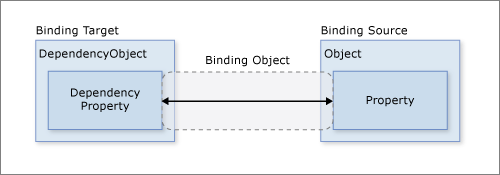
\includegraphics[height=3cm]{ressources/images/basic-data-binding-diagram.png}
    \caption{La liaison de données}
\end{figure}

Grâce à cette caractéristique, il est facile d'utiliser les changements apportés à la partie modèle de MVVM pour conduire des changements dans l'affichage de l'interface. Plus précisément, lors du développement du \texttt{PowerEye}, j'utilise des informations de données telles que les chemins sélectionnés et les fichers ouverts comme la partie modèle. Et le modèle de vue contient la partie modèle et les fonctions de contrôle des événements. Enfin, l'apparence de l'interface apparaît comme la vue. En outre, pour rendre la structure global plus claire, j'ai établi une distinction entre la couche de présentation et la couche d'applications.
\begin{figure}[H]
    \centering
    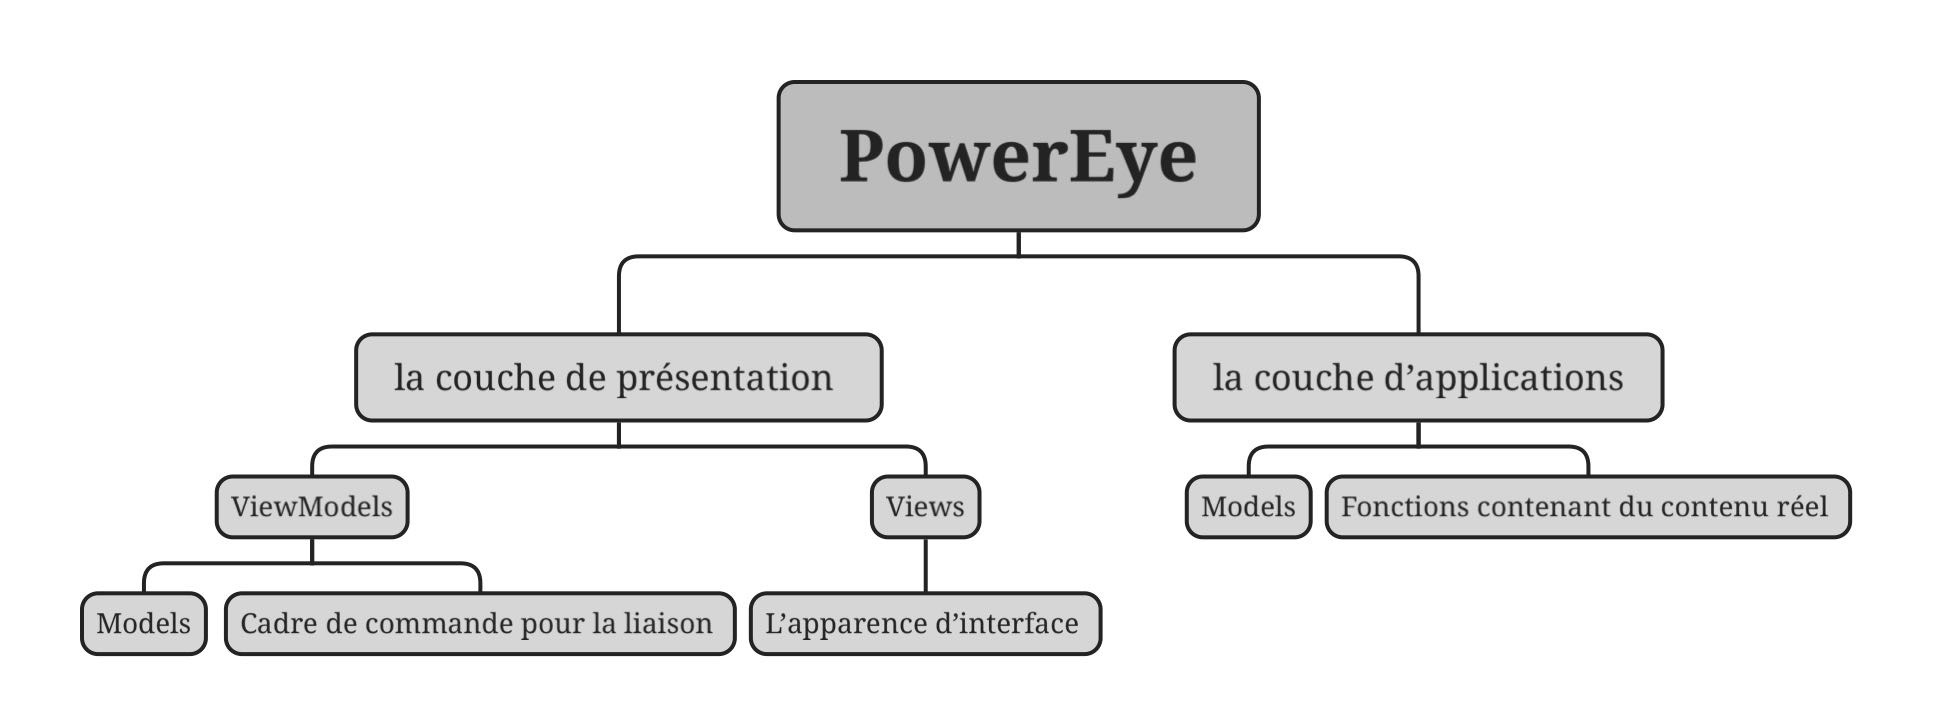
\includegraphics[height=5cm]{ressources/images/PowerEye_Structure.jpg}
    \caption{La structure globale du PowerEye}
\end{figure}

\subsubsection{Avantages de ce choix}
L'utilisation de ce modèle de conception facilite grandement l'ensemble du processus de développement. Premièrement, il sépare le développement de l'apparence de l'interface de l'ensemble. Une fois l'apparence de l'interface développée, l'adaptation des données peut être réalisée en modifiant simplement la source de la liaison de données. De plus, nous pouvons réutiliser le modèle de vue pour des interfaces similaires. Enfin, comme la couche d'application est séparée, il est possible d'appeler directement des fonctions qu'elle contient pour tester.

\subsection{Structure des données}
Les données font partie du modèle dans le cadre de MVVM, je les ai également conçu pour répondre aux besoins. Pour chaque module, j'ai créé une sous-classe avec une liste pour stocker les instances qui ont été créées. Afin que les différentes interfaces d'un même module puissent être enregistrées dans la même liste, j'ai créé une classe de base. Enfin, les classes de chaque interface héritent simplement de la classe de base et modifiée différemment en fonction des besoins. En outre, la classe de base doit hériter de la classe \texttt{BindingBase} pour implémenter la fonctionnalité de notification de l'interface lorsqu'une propriété est changée. Et voici un aperçu de la structure des données.

\begin{figure}[H]
    \centering
    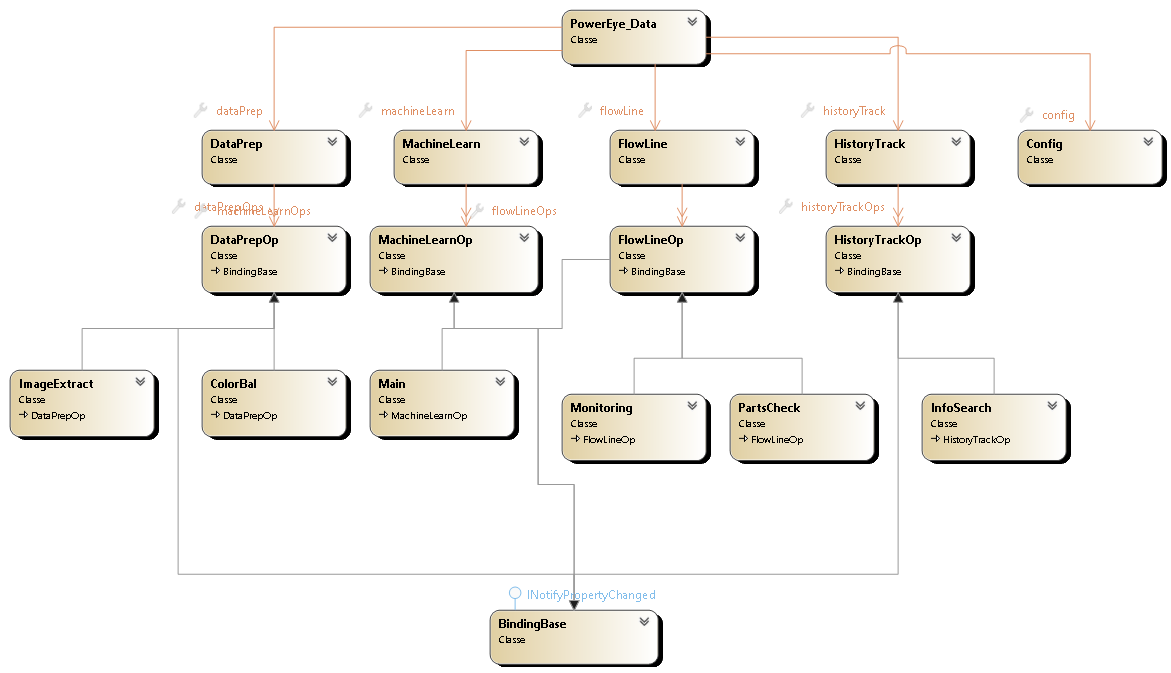
\includegraphics[height=9cm]{ressources/images/PowerEye_Data.png}
    \caption{La structure des données du PowerEye}
\end{figure}
\subsection{Disposition de l'interface graphique}
Après avoir présenté la partie du modèle, j'aimerais expliquer la conception de la disposition de l'interface graphique, c'est-à-dire la partie concernant la vue dans le cadre de MVVM. La \hyperref[fig:target]{\textsc{figure 2}} montre le style d'interface du \texttt{PowerEye}, qui semble se composer de trois parties. Mais ce n'est pas vraiment ce que j'ai fait avec l'interface au début. Au départ, j'ai choisi le \texttt{Tabcontrol} pour séparer les modules et les développer à partir de là. L'interface conçue à ce moment-là est illustrée ci-dessous.
\begin{figure}[H]
    \centering
    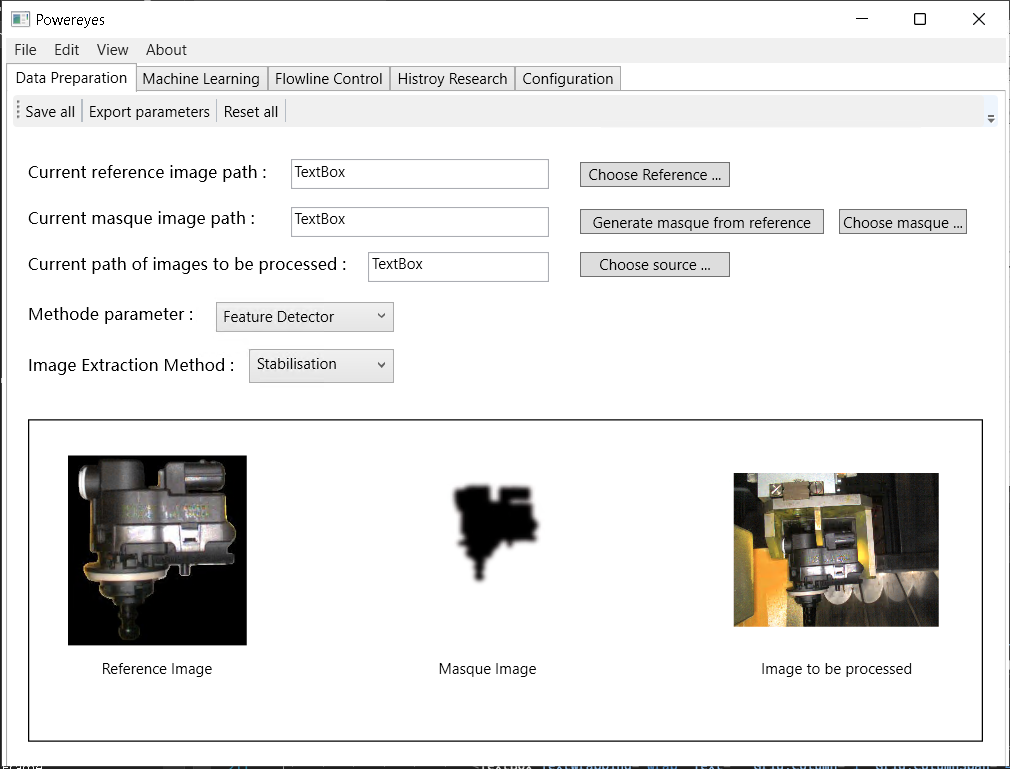
\includegraphics[height=8cm]{ressources/images/Interface_original.png}
    \caption{La Conception initiale de l'interface}
\end{figure}

Cependant, le problème est double: d'une part, chaque module n'a pas nécessairement une seule fonction, et les combiner dans une interface unique aurait l'air encombré. D'autre part, avec cette approche, le développement de toutes les interfaces des modules se fait dans le même ficher, ce qui réduit la lisibilité du code.

J'ai donc finalement choisi d'abandonner cette solution et d'utiliser 
\texttt{Contentcontrol} pour la disposition de l'interface. Plus précisément, j'ai divisé l'interface globale en trois parties: la barre des modules, la barre des fonctions et la fenêtre principale. En sélectionnant le module, différentes barres de fonctions s'affichent, puis la fenêtre principale est affichée en cas de sélection de la fonction. Et grâce à la caractéristique du \texttt{Contentcontrol}, nous pouvons injecter l'interface en tant que contrôle, ce qui permet le développement indépendant des différentes parties. La disposition finale de l'interface est illustrée ci-dessous.
\begin{figure}[H]
    \centering
    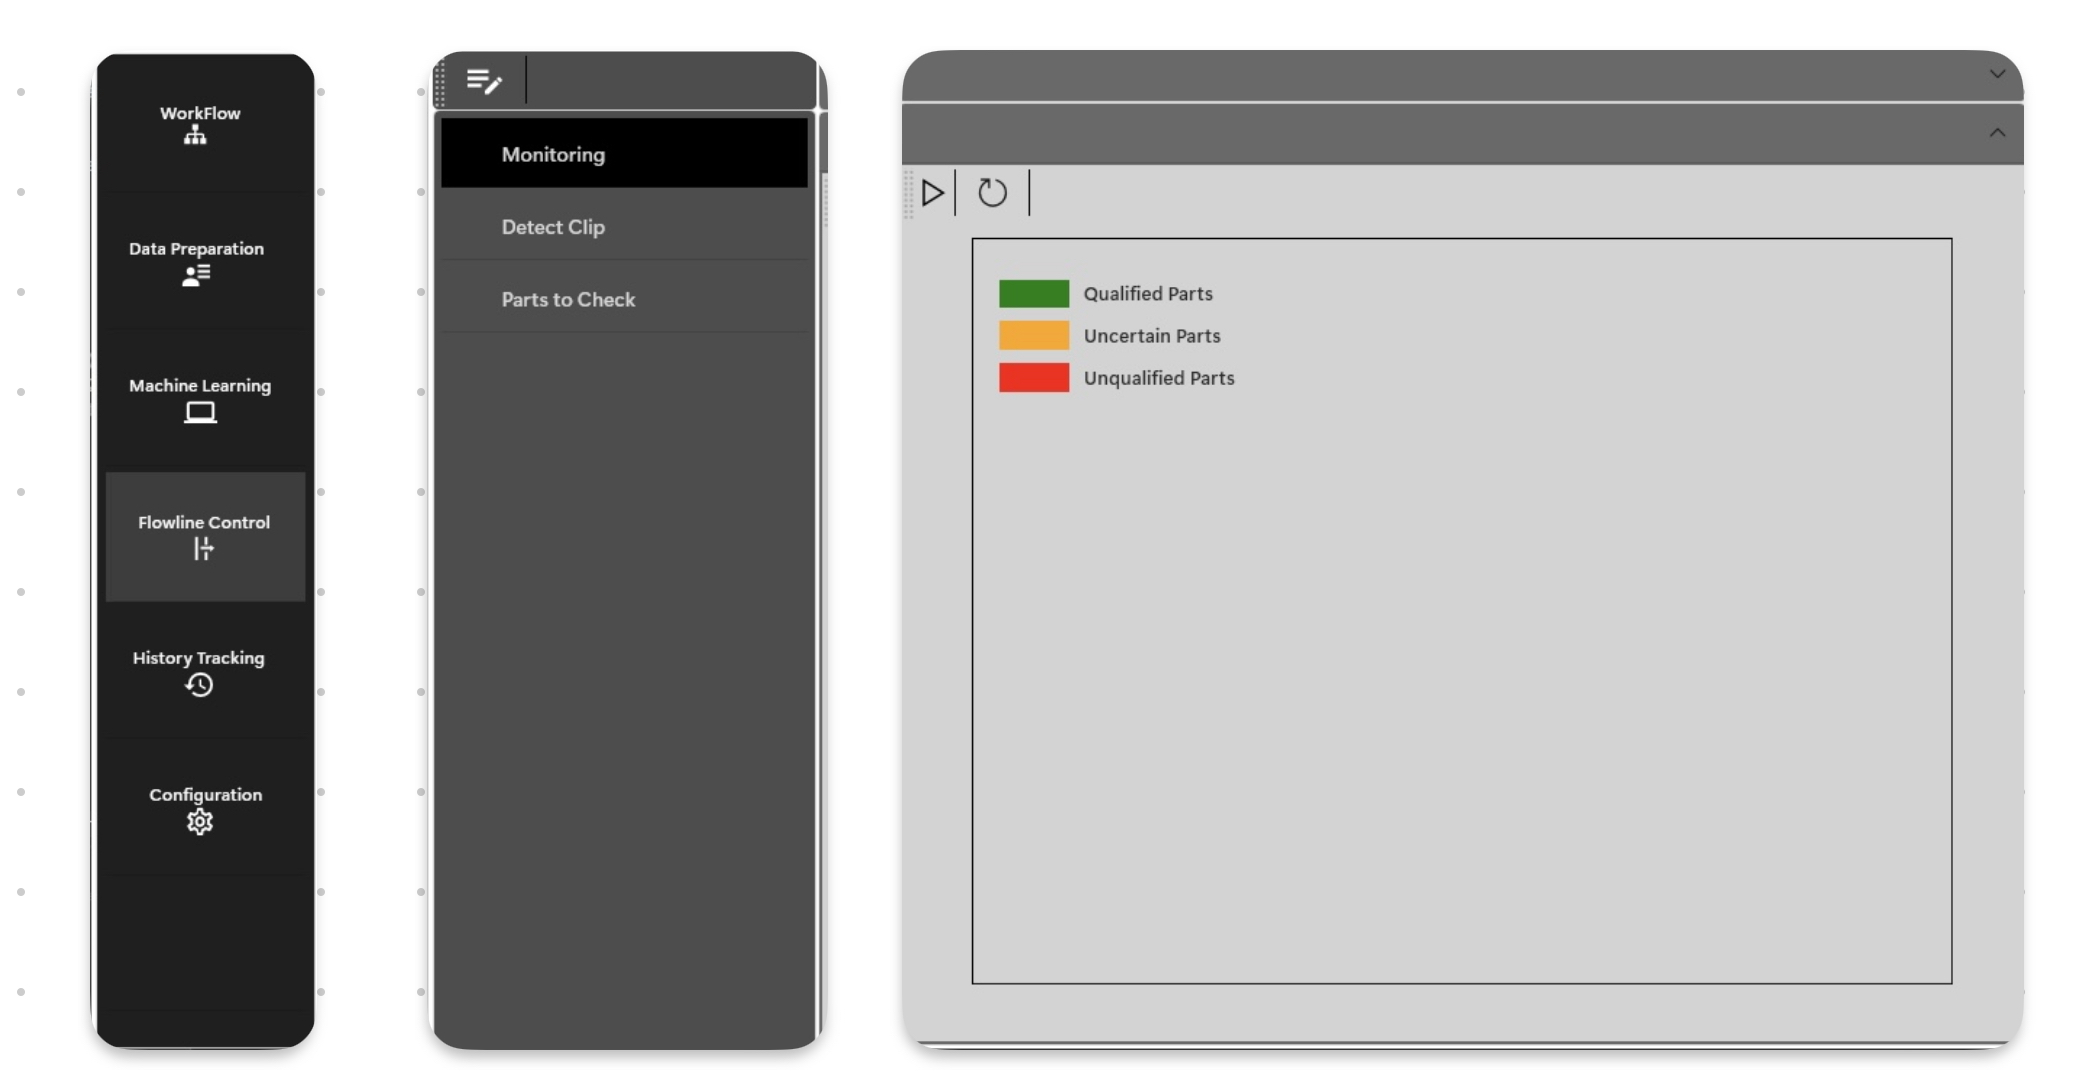
\includegraphics[height=8cm]{ressources/images/PowerEye_Disposition.jpg}
    \caption{ La disposition finale de l’interface}
\end{figure}

Dans la partie de la fenêtre principale, compte tenu du fait que la réalisation de nombreuses fonctions nécessite la sélection du chemin d'accès au ficher et d'autres configurations, j'ai également fait la conception correspondante. L'\texttt{Expander} est utilisé pour diviser la fenêtre en deux parties, la partie supérieure pour les choix de configuration et la partie inférieure pour les fonctionnalités. La figure suivant montre spécifiquement la fenêtre principale. 
\begin{figure}[H]
    \centering
    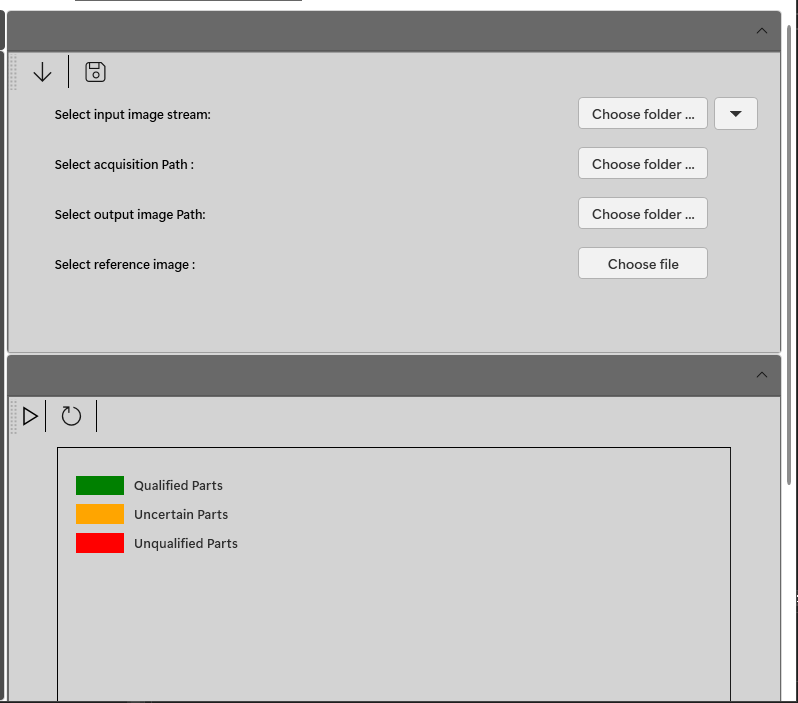
\includegraphics[height=8cm]{ressources/images/fenetre_disposition.png}
    \caption{la fenêtre principale}
\end{figure}

\section{Multiples modules pour PowerEye}
Après l'introduction générale du \texttt{PowerEye}, cette section va le présenter en détail à partir de chaque module.

\subsection{Préparation des données}
Le traitement des données étant une condition préalable à la formation au modèle, un module a également été spécialement conçu dans \texttt{PowerEye} pour mettre en œuvre les fonctions correspondantes. Dans ce module, nous avons actuellement développé deux interfaces entièrement fonctionnelles, à savoir l'extraction d'images et l'ajout du bruit de perlin. 
\subsubsection{Extraction d'images}
L'objectif de cette interface est d'extraire le contour de la pièce sur le photo de la ligne d'assemblage. Lorsque j'ai commencé à développer \texttt{PowerEye}, une fonction qui utilise le \texttt{feature matching} pour réaliser cet objectif a déjà été développée. Donc ma tâche principale a consisté à l'intégrer dans l'interface et à y apporter des améliorations. 

Lors de la conception de l'interface graphique pour cette fonctionnalité, j'ai suivi l'idée générale selon laquelle la partie supérieure de l'interface est utilisée pour la sélection de la configuration. Dans la partie inférieure de l'interface, j'ai conçu une barre de progression et une fenêtre pour montrer l'image avant et après le traitement. 
\begin{figure}[H]
    \centering
    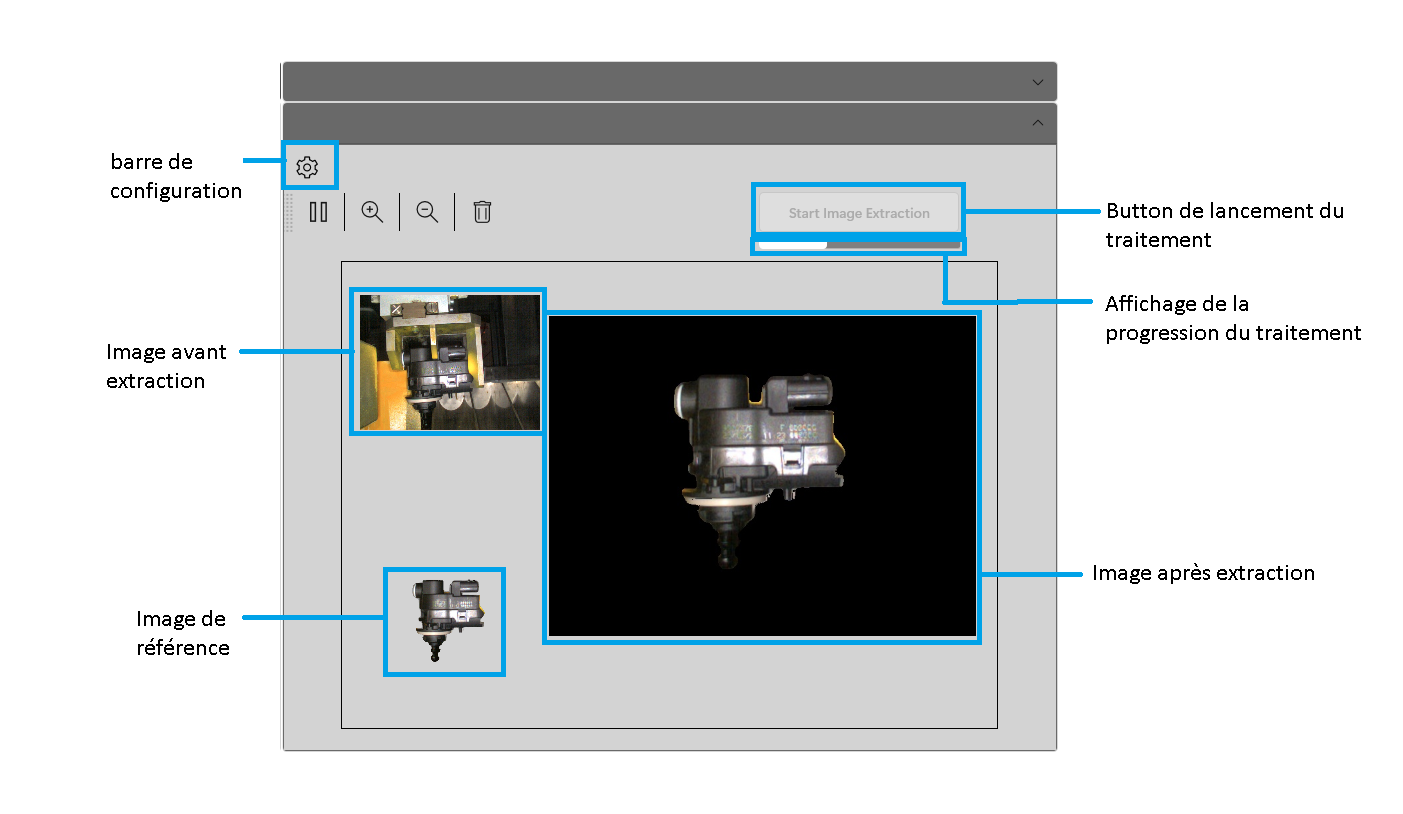
\includegraphics[height=8.5cm]{ressources/images/imageExtract.png}
    \caption{l'interface graphique d'extraction d'images}
\end{figure}

En ce qui concerne l'intégration de la fonctionnalité d'extraction développée, j'ai résolu deux problèmes principaux. D'une part, la fonction est développée en C++, tandis que l'interface est développée en C\#, il faut donc choisir la bonne méthode pour l'appeler. En final, j'ai choisi d'utiliser la même méthode que l'interface prototype, en appliquant le ficher \texttt{dll} pour l'importation et l'exportation des fonctions. D'autre part, c'est un problème très courant dans le développement d'interface graphiques est de savoir comment exécuter la fonction sans bloquer l'interface graphique. Donc le \texttt{thread} est utilisé pour résoudre ce problème. J'ai intégré la fonction extraite dans un \texttt{thread} et appliqué \texttt{FileWatcher} pour détecter les images ajoutée au répertoire afin de les afficher. Plus précisément, il fonctionne de la manière suivante : 
\begin{enumerate}
    \item Après de cliquer sur le bouton de démarrage, un nouveau \texttt{thread} est créé pour exécuter la fonction d'extraction d'image. 
    \item \texttt{FileWatcher} surveille toujours le répertoire de destination et détecte si les images traitées ajoutées sont occupées.
    \item Lorsque l'image n'est plus occupée, modifie le propriété de la source de liaison dans le \texttt{thread} principal pour l'afficher.
\end{enumerate}

\subsubsection{Ajout du bruit de perlin}
L'objectif de cette interface est d'ajouter un masque de bruit à l'image pour générer des pièces comportant des défauts. Comme dans la partie précédent, il existe déjà une fonction permettant d'ajouter des masques de bruit, développée à l'aide de python. L'idée de conception et la manière de fonctionner de cette partie sont similaires à la précédente, que je vais brièvement présenter ici. L'interface graphique est présentée comme ci-dessous. 
\begin{figure}[H]
    \centering
    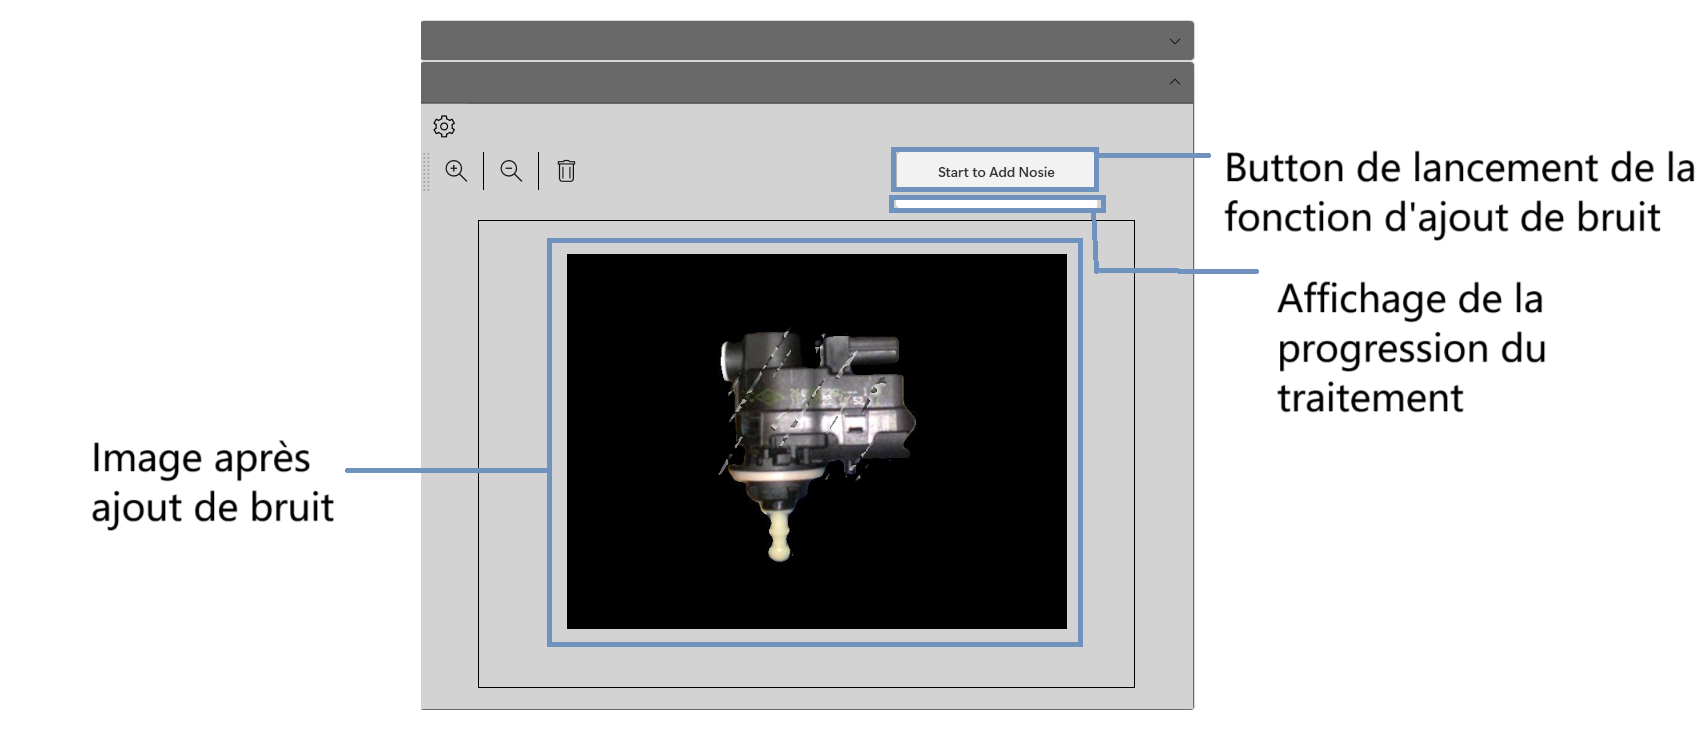
\includegraphics[height=8cm]{ressources/images/perlin_noise.png}
    \caption{l'interface graphique d'ajout du bruit}
\end{figure}

Et dans la section, je vais me concentrer sur la méthode d'appel python et sur une amélioration que j'ai réalisée. Pour l'appel au module python, je me réfère à l'implémentation de l'interface prototype. La classe \texttt{process} en C\# me permet d'exécuter python et de passer le script à lancer comme les paramètres de démarrage. Et dans la mise en œuvre, j'ai également encapsulé le processus python, y compris les valeurs d'entrée et de sortie, dans une classe pour le réutiliser dans le module d'apprentissage automatique. 

En termes d'améliorations, la fonction d'ajout de bruit nécessite trois paramètres d'entrée: une image de la pièce, un masque de bruit et un masque de forme. 
\begin{figure}[H]
    \centering
    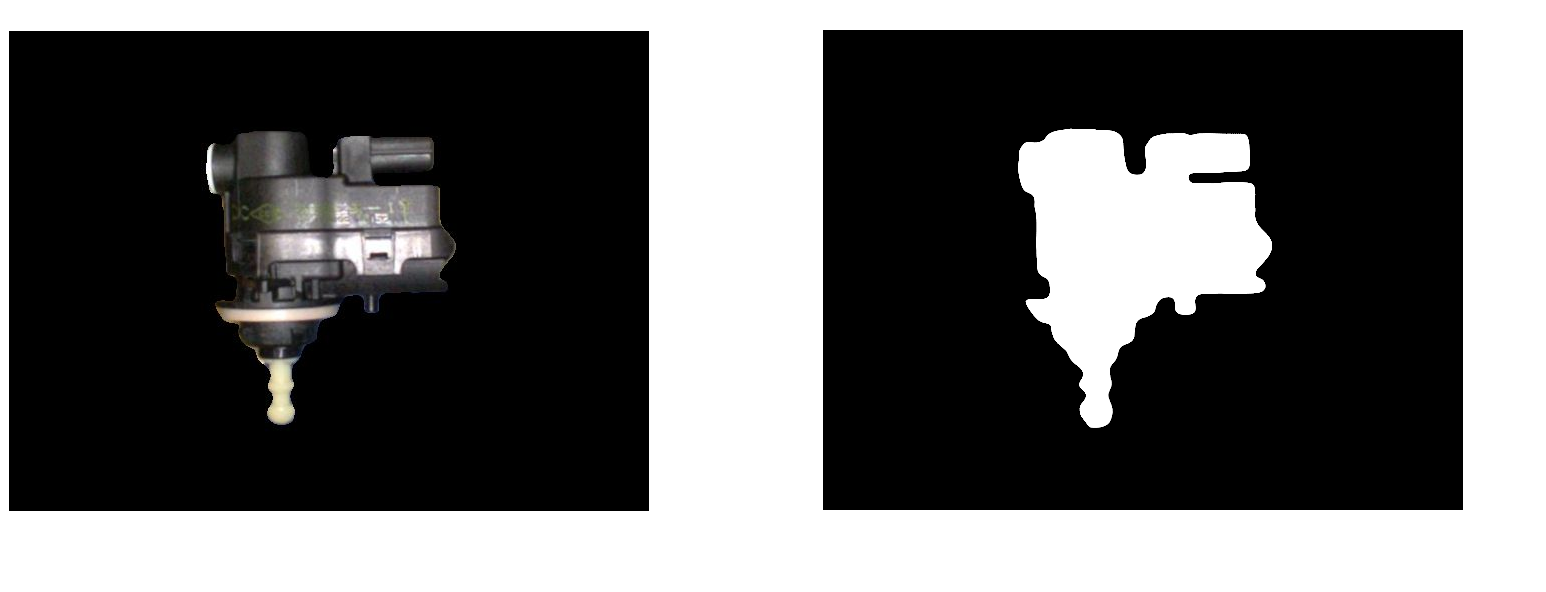
\includegraphics[height=4cm]{ressources/images/input_perlin.png}
    \caption{trois paramètres d'entrée}
\end{figure}
Mais en effet, il n'est pas difficile d'obtenir le masque de forme d'une pièce à partir de l'image initial. Par conséquent, j'ai développé la fonction pour générer les masques de forme afin de réduire la paramètre d'entrée. Les étapes pour réaliser cette fonction sont les suivantes: 
\begin{enumerate}
    \item Chargement et conversion de l'image d'entrée en niveaux de gris et Application d'un flou gaussien.
    \item Calcul de la magnitude et de la direction du gradient à l'aide de l'algorithme de Scharr.
    \item Normalisation de la magnitude du gradient dans la plage [0, 255].
    \item Opération de fermeture morphologique et recherche du plus grand contour d'arête.
    \item Générer et exporter des masques transparents avec des contours de remplissage maximaux.
\end{enumerate}

Après avoir terminé cette partie de l'amélioration, le module de préparation des données est désormais plus robuste, ce qui permet de passer au module d'apprentissage automatique qui utilise les données.

\subsection{Apprentissage automatique}


\subsection{Contrôle de la chaîne d'assemblage} 
Ce module, qui est l'application la plus importante de tout le logiciel, permet de détecter les images des pièces sur la ligne d'assemblage et de sauvegarder les données.

\subsubsection{Surveillance de la ligne d'assemblage}
L'idée de cette fonction est d'utiliser le modèle entraîné pour inspecter chaque image de pièce et d'afficher les résultats de l'inspection dans l'interface. Mais pendant le développement, il était impossible d'accéder aux capteurs dans la scène réelle. J'ai donc utilisé un processus qui copie les images dans un répertoire toutes les cinq secondes comme une alternative. 

Dans la conception de l'interface, j'ai choisi d'utiliser différentes couleurs pour indiquer si le pièce est qualifiée ou non, un peu comme le voyant d'avertissement, et afficher l'image de ce pièce. L'interface graphique conçue est illustrée ci-dessous.
\begin{figure}[H]
    \centering
    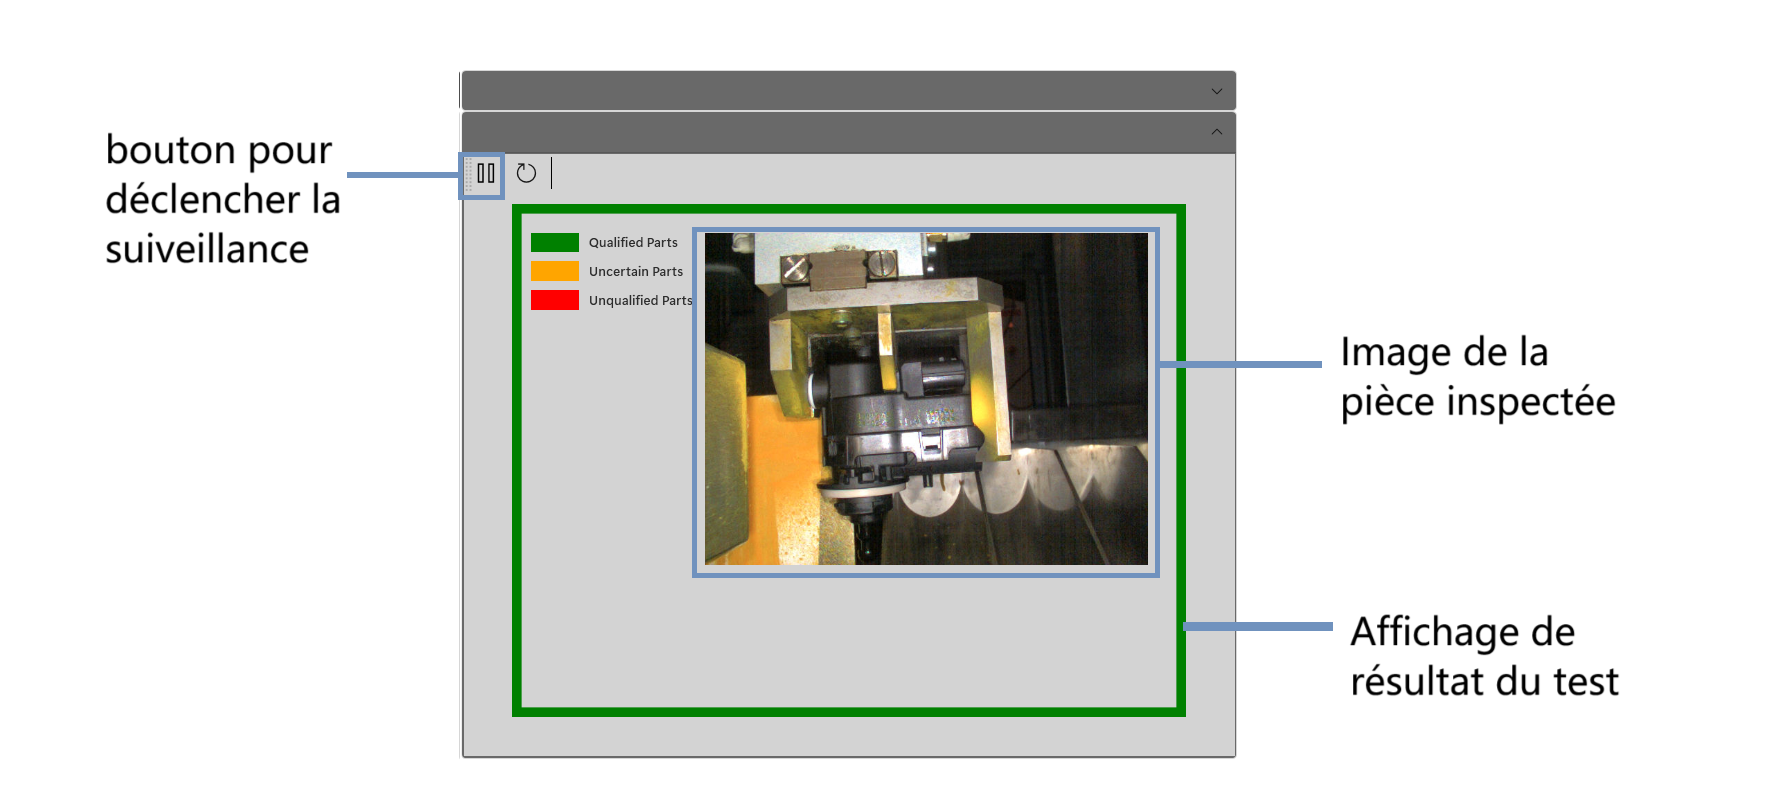
\includegraphics[height=8cm]{ressources/images/monitoring.png}
    \caption{Interface graphique de la surveillance de la ligne d'assemblage}
\end{figure}

 Les pièces dont le score est inférieur à 90 sont considérées comme non qualifiées, celles dont le score est supérieur ou égal à 95 sont considérées comme qualifiées, et celles dont le score est compris entre 90 et 95 doivent être testées à nouveau manuellement. La réalisation de la fonctionnalité utilise la même approche que dans la section précédente, en utilisant  un \texttt{thread} et \texttt{FileWathcer} pour assurer l'interaction de l'interface.

\subsubsection{Sauvegarde des données de pièces}
Une fois la pièce analysée, ses données sont sauvegardées dans une autre interface. Dans cette interface, j'ai conçu trois listes pour stocker les données des différents types de pièces, y compris son temps de production, le nombre de points gagnés et le chemin où l'image est sauvegardée. 
\begin{figure}[H]
    \centering
    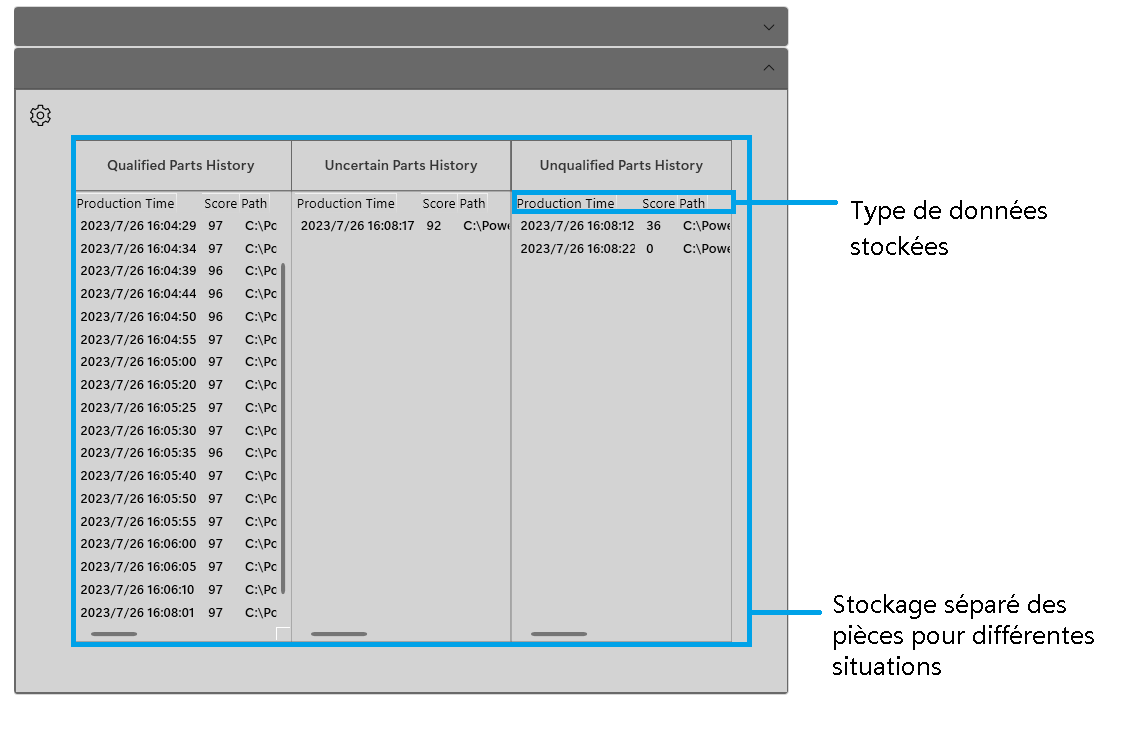
\includegraphics[height=8cm]{ressources/images/check_parts.png}
    \caption{Interface graphique pour le stockage des données relatives aux pièces }
\end{figure}

Et pour les pièces dont la qualification n'est pas certaine, vous pouvez les vérifier manuellement en cliquant sur la liste. Une nouvelle fenêtre apparaît alors et l'état de la pièce peut être vérifié en faisant glisser l'image vers la gauche ou la droite. 
\begin{figure}[H]
    \centering
    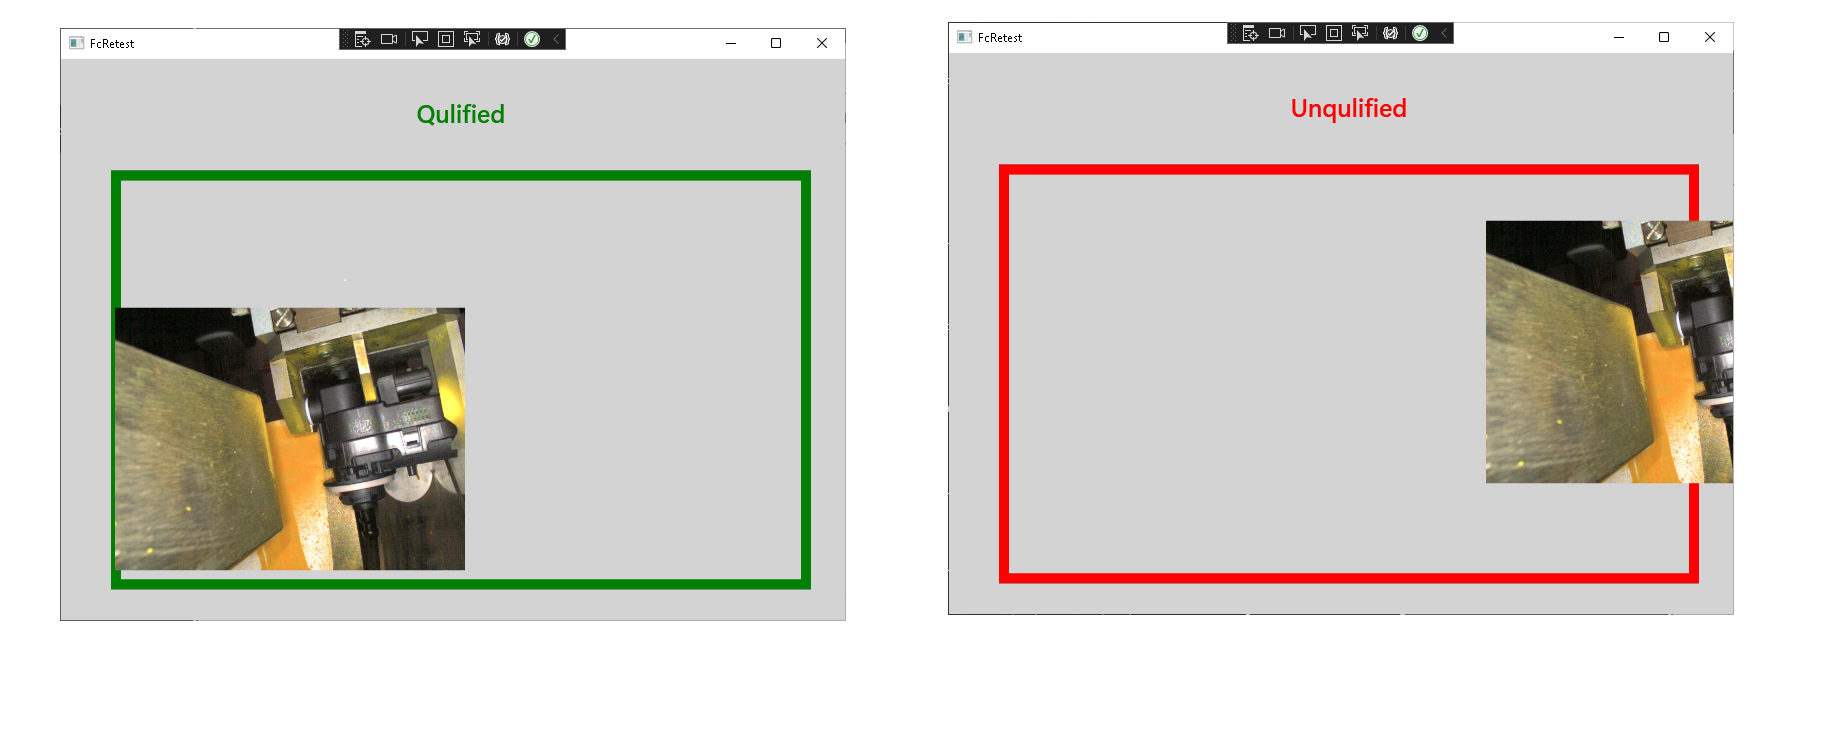
\includegraphics[height=6cm]{ressources/images/check_manuel.png}
    \caption{Interface graphique pour la vérification manuelles}
\end{figure}

\subsection{Suivi des données relatives aux pièces}
Le module est conçu pour une utilisation à long terme et retracer les données de la pièce précédente enregistrées dans des fichiers \gls{Excel}. 

\subsubsection{Interroger les données historiques}
L'idée de cette fonction est d'afficher le fichier \gls{Excel} sélectionné dans l'interface, d'effectuer une recherche par mot-clé et d'enregistrer les résultats de la recherche. 

Dans la conception de l'interface, J'utilise une grille de données pour afficher les données d'un fichier \gls{Excel}, une barre de sélection pour choisir le type de données à filtrer et une zone de texte pour saisir des mots-clés. 
\begin{figure}[H]
    \centering
    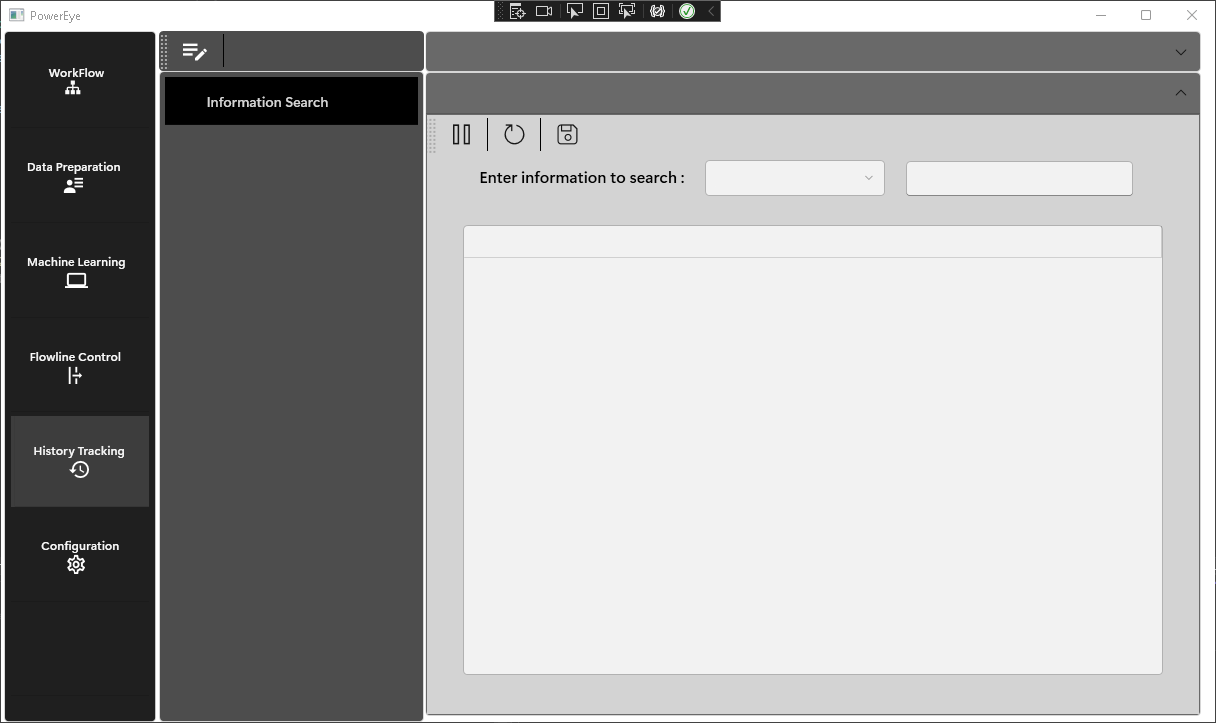
\includegraphics[height=9cm]{ressources/images/information_search.png}
    \caption{Interface graphique pour l'interrogation de l'historique }
\end{figure}

Afin de lire le fichier Excel, une extension \texttt{ClosedXML} est utilisée, ce qui me permet d'obtenir le contenu du fichier par chemin et de le stocker dans la classe \texttt{DataTable}.  J'ai ainsi créé deux fonctions pour convertir un chemin d'accès en \texttt{DataView} contenant un tableau et un chemin d'accès en une liste contenant les lignes d'en-tête d'un tableau. Et pour obtenir cette fonction de filtrage, la propriété \texttt{RowFilter} de \texttt{DataView} est tout à fait appropriée, il suffit de changer sa valeur en fonction de différents mots-clés pour modifier le contenu de l'affichage. Enfin, pour pouvoir enregistrer le tableau filtrée, il est nécessaire de créer une classe \texttt{DataView} qui supprime effectivement les données en fonction du \texttt{RowFilter} et de la convertir en utilisant l'extension. 

\subsection{Configuration des données globales}
Le module est principalement conçu pour permettre aux développeurs de compléter la sélection de la configuration de plusieurs modules directement par l'importation de fichiers de configuration afin de faciliter les tests. Par ailleurs, dans les scénarios d'application pratique, la construction de l'environnement d'exécution peut également être facilitée par une configuration globale.

\subsubsection{Affichage des informations sur la configuration actuelle}
L'interface est conçue pour permettre aux développeurs de visualiser la configuration globale actuelle du logiciel. Dans la section précédente de l'introduction générale, j'ai expliqué la structure de données qui compose \texttt{PowerEye}, consistant en les listes d'exemples de composants pour chaque interface de chaque module. Je n'ai donc besoin que d'afficher cette classe de données sur l'interface. Dans le choix de la méthode, j'ai choisi d'afficher le contenu après la sérialisation \gls{XML}, car cela convient mieux à ma réalisation ultérieure de la fonction d'importation et d'exportation, d'autre part, c'est plus pratique que de reconstruire toute la fonction \texttt{tostring} de données. En outre, j'ai développé la fonctionnalité de sérialisation afin de sauvegarder les configurations actuelles. 

En termes de conception de l'interface graphique, cette section est plutôt simple, avec une zone de texte pour afficher les informations de configuration et un bouton pour sauvegarder la configuration actuelle.
\begin{figure}[H]
    \centering
    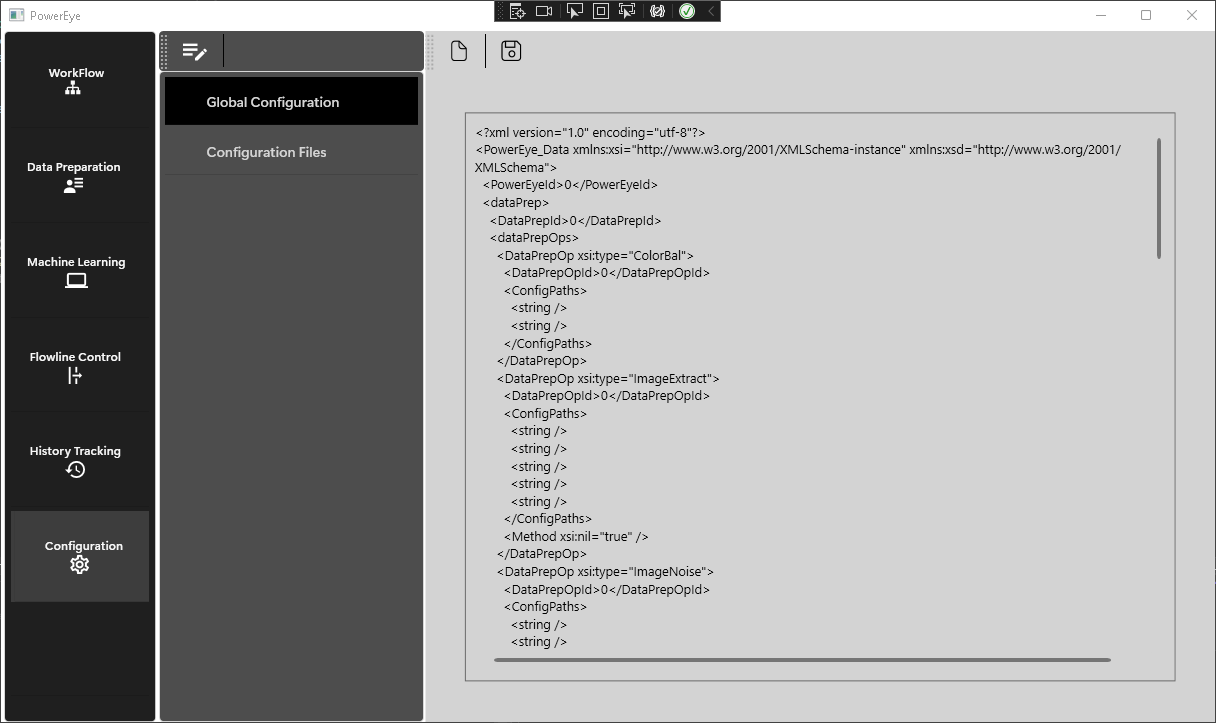
\includegraphics[height=8cm]{ressources/images/global_configuration.png}
    \caption{Interface graphique montrant la configuration globale}
\end{figure}

\subsubsection{Importation de configuration}
Cette interface est conçue pour appliquer les configurations précédemment sauvegardées à l'ordinateur. En utilisant la désérialisation \gls{XML}, nous pouvons reconstruire le fichier sauvegardé en classe de données de \texttt{PowerEye}. Dans la classe de données, j'ai implémenté une fonction de copie pour chaque sous-classe afin de remplacer la valeur par la valeur générée par le fichier. 


\begin{figure}[H]
    \centering
    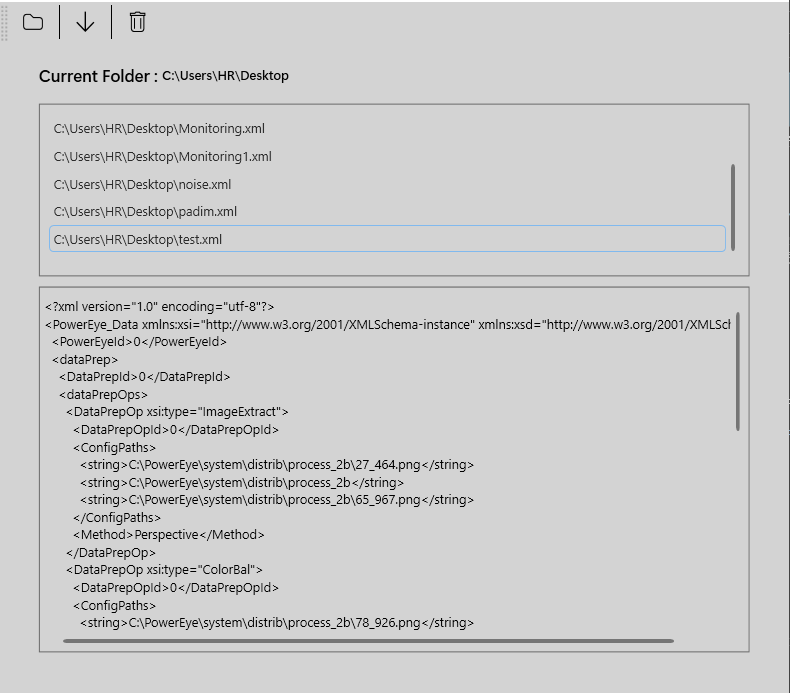
\includegraphics[height=8cm]{ressources/images/configuration_files.png}
    \caption{Interface graphique montrant la configuration globale}
\end{figure}









\subsection{Flux de travail personnalisés}
\section{Fonctions en dehors du corps principal}
Dans le dernière partie de mes réalisations, je vais présenter deux fonctionnalités que j'ai développées en dehors du corps principal du logiciel. Bien que ces deux fonctions ne constituent pas directement le logiciel, elles contribuent au processus de tests.
\subsection{Affichage de l'appel de fonction}
\begin{figure}[H]
    \centering
    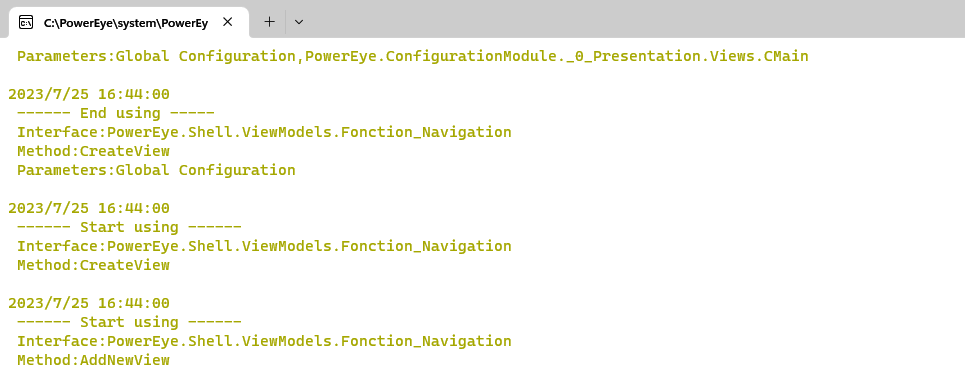
\includegraphics[height=7cm]{ressources/images/aop_log.png}
    \caption{l'interface graphique d'ajout du bruit}
\end{figure}
\subsection{Exécution de la chaîne de caractères comme un script}


\chapter{Conclusion}
Mon stage a été entièrement consacré à la poursuite du développement de \texttt{PowerEye}.Ce logiciel développé par Deltacad dans le cadre d’un projet de recherche en partenariat avec les laboratoires d’UTC et AML Systems, est destiné à être utilisé pour détecter des anomalies sur les objets sortant de chaînes de productions avec vision par ordinateur. 

Avant de commencer mon stage, le logiciel était dans sa phase de prototypage. Il contient des fonctionnalités développées par le stagiaire précédent, ainsi qu'un module d'apprentissage automatique développé par les laboratoires d'UTC. Lorsque j'ai terminé mon stage, il disposait d'une interface graphique mature, de modules clairement différenciés et de fonctionnalités rationalisées. Plus précisément, au cours de mon stage, j'ai non seulement achevé le développement d'une toute nouvelle IHM pour \texttt{PowerEye}, mais j'ai également transféré toutes les fonctionnalités de l'interface prototype vers la nouvelle interface et j'en ai amélioré une grande partie. De plus, j'ai réalisé le développement du module de configuration, du module de suivi des pièces, et de deux fonctions hors du corps principal du logiciel. Avec ma contribution, \texttt{PowerEye} passe progressivement du stade du prototype à celui de l'optimisation.

À l'avenir, j'espère que powereye aura des fonctionnalités plus complètes, y compris la partie équilibrage des couleurs pour laquelle j'ai développé l'interface mais pas le fonctionnalité. Par ailleurs, j'aimerais que l'adaptation aux différentes pièces de l'entreprise soit réalisée, car pour l'instant, nous ne testons que les données de AML Systems. 

Mais de toutes façons, cette expérience de stage m'a beaucoup touchée. Ce stage m'a donné l'occasion de travailler dans une entreprise et de participer à un projet à long terme, ce qui m'a permis de comprendre comment organiser mon travail et discuter des détails avec mes collègues. D'autre part, en tant qu'étudiant qui vient d'arriver en France pour un an, cette expérience me sert également d'expérience d'échange international, me permettant de sentir l'environnement de travail français et de communiquer avec les autres avec plus d'assurance. 

Au cours de mon stage, j'ai également mis en évidence certaines insuffisances. En raison de mon manque de compréhension du développement WPF, j'ai utilisé un cadre trop complexe au début de mon développement, ce qui m'a fait perdre du temps à e résoudre ce problème. 

Cependant, ce stage a renforcé ma confiance dans le choix d'un poste en recherche et développement et m'a permis de m'intéresser davantage au traitement d'images et à la conception d'interfaces de programmation. Je peux aussi comprendre que j'ai la capacité de développer des projets de manière indépendante, ce qui me permet d'envisager l'avenir de l'apprentissage et du travail avec optimisme.
\printglossaries
\printbibliography[title={Bibliographie},heading={bibintoc}]
\label{LastPage}
\end{document}
\grid